\documentclass{scrartcl}

\usepackage[ngerman]{babel}

\usepackage[margin=0cm]{geometry}
\usepackage[hidelinks]{hyperref}
\usepackage{csquotes}

\usepackage{fontspec}
\setsansfont{Titillium SemiBold}
\usepackage{fontawesome}

\usepackage{tikz}
\usetikzlibrary{calc}

\usepackage{graphicx}
\usepackage{xcolor}

\definecolor{fsfw-cyan}{HTML}{28ADB8}
\definecolor{fsfw-violett}{HTML}{654BC7}
\definecolor{fsfw-green}{HTML}{6BBB00}

\begin{document}

\begin{tikzpicture}[overlay,remember picture]

  % background
  \node[anchor=north,overlay,fill=black!10!white,minimum width=\textwidth, minimum height=\textheight] at ($(current page.north)$) {};

  % top
  \node[anchor=north,fill=white,inner sep=0cm,rounded corners=3mm] (top)
  at ($(current page.north) + (0,-1.07)$)
  {
    \begin{tikzpicture}
      \useasboundingbox[clip] (-9.53,5) rectangle (9.53,-5.1);

      \node[anchor=north,overlay] at (0,5.0) {
        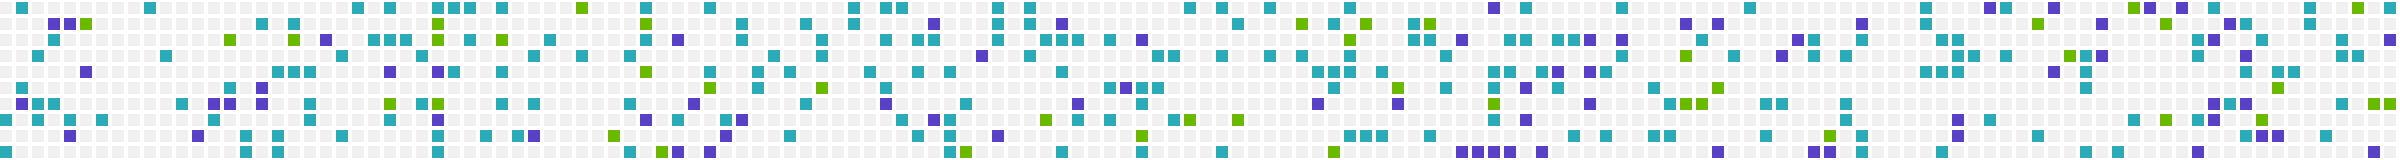
\includegraphics[width=1.0\textwidth]{banner.png}
      };

      \node[anchor=north,overlay] at (0,-3.7) {
        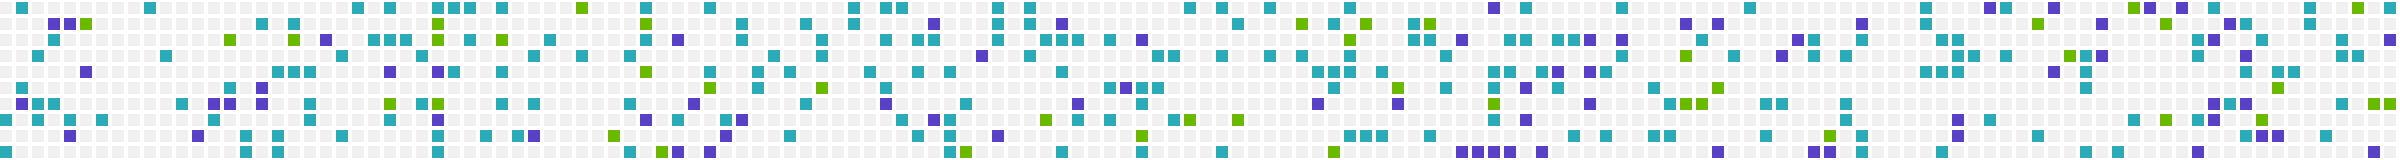
\includegraphics[width=1.0\textwidth]{banner.png}
      };

      \node[scale=3,at={(-0.5,3.3)}]{%
        \textbf{\textsf{\color{fsfw-cyan}\large%
              Schöne Abschlussarbeit?}}
      };
      \node[scale=3,at={(0,1.3)}]{%
        \textbf{\textsf{\color{fsfw-violett}\Huge%
            Mit \textrm{\LaTeX}!}}};
      \node[scale=3,at={(2,-2.0)}]{%
          \textbf{\textsf{\large\textcolor{fsfw-cyan}{%
              Hier gibt's Hilfe.}}}};
    \end{tikzpicture}
  };

  % middle
  \node[fill=white,anchor=north,inner sep=0cm, rounded corners=3mm] (middle)
  at ($(top.south) + (0,-1.07)$){
    \begin{tikzpicture}
      \useasboundingbox (-9.55,5.75) rectangle (9.55,-5.5);
      \node[anchor=north] at (0,5.7) {
        \parbox[t][11.25cm][t]{18cm}{
          \begin{center}
            \Huge\color{fsfw-violett}
            \textbf{\textsf{\textrm{\LaTeX}/LibreOffice Sprechstunde}}\\[1ex]
            \LARGE
            \color{black}
            \textsf{Direkte Hilfe bei Problemen mit \textbf{\textrm{\LaTeX}} und LibreOffice.}
          \end{center}

          \bigskip
          \bigskip

          \centering

          \parbox[t][6cm]{8cm}{
            {\Huge\textbf{\textsf{\textcolor{fsfw-green}{Termine}}}}

            \LARGE
            \null\hspace*{0.1em}\parbox{0.8\linewidth}{\sf%
              Mittwoch, 27.04.2016\\
              Mittwoch, 25.05.2016\\
              Mittwoch, 22.06.2016\\
              Mittwoch, 27.07.2016\\
              Mittwoch, 24.08.2016\\
              Mittwoch, 28.09.2016
            }
          }
          \parbox[t][6cm]{6cm}{
            \parbox[t][3.045cm]{\linewidth}{
              {\Huge\textbf{\textsf{\textcolor{fsfw-green}{Ort}}}}

              \vspace*{\baselineskip}

              \LARGE
              \hspace*{0.1em}\textsf{SLUB, Raum -2.115}
            }\\
            \parbox[t][3.5cm]{\linewidth}{
              {\Huge\textbf{\textsf{\textcolor{fsfw-green}{Zeit}}}}

              \vspace*{\baselineskip}

              \LARGE
              \hspace*{0.1em}\textsf{ab 19:00 Uhr}
            }
          }

          \vfill

          \begin{center}
            \large
            \textbf{\textsf{%
                \faicon{home}\,
                \href{https://fsfw-dresden.de/sprechstunde}%
                {\textcolor{fsfw-cyan}{https:/\hspace*{-0.1em}/fsfw-dresden.de/sprechstunde}} \quad
                \faicon{envelope}\,
                \href{mailto:sprechstunde@fsfw-dresden.de}
                {\textcolor{fsfw-cyan}{sprechstunde@fsfw-dresden.de}}}
            }
          \end{center}
        }
      };
    \end{tikzpicture}
  };

  % footer
  \node[anchor=south,fill=white,inner sep=0cm, rounded corners=3mm] (bottom)
  at ($(current page.south) + (0,1.07)$) {\textbf{\textsf{
    \begin{tikzpicture}
      \useasboundingbox (-9.53,2.5) rectangle (9.53,-1.5);
      \node[rectangle,minimum height=4.0cm,minimum width=19cm] at (0, -1.5) {
        \parbox[b][4.0cm]{4.2cm}{
          
\includegraphics[origin=cc,width=4cm]{sitelogo.pdf}
        }
        \parbox[b][3.5cm]{9.4cm}{
          \null\vfill
          \centering
          \Large
          Hochschulgruppe für\\
          Freie Software und Freies Wissen\\
          \medskip
          \href{https://fsfw-dresden.de}{\textcolor{fsfw-cyan}{https:/\hspace*{-0.1em}/fsfw-dresden.de}}
          \vfill\null
        }
        \parbox[b][3.5cm]{4.2cm}{
          \null\vfill\centering
          \vspace*{-1.3\baselineskip}
          {\normalsize \textmd{In Kooperation mit der}}
          \vspace*{0.7\baselineskip}\\
          
\includegraphics[origin=cc,width=4cm]{Logo-SLUB.jpg}
          \vfill\null
        }
      };
    \end{tikzpicture}
  }}};
\end{tikzpicture}

\newpage

\end{document}

%%% Local Variables:
%%% mode: latex
%%% TeX-master: t
%%% TeX-engine: luatex
%%% End:
